\documentclass{beamer}
\usetheme{metropolis}

\usepackage{tikz}
\usetikzlibrary{shapes.geometric, arrows}
\tikzstyle{service} = [rectangle, minimum width=2cm, minimum height=1cm, text centered, draw=black, fill=white]
\tikzstyle{flow} = [thick,->,>=stealth]
\tikzstyle{depends} = [thick,-,>=stealth]

\newcommand\TBox[3][]{%
  \tikz\node[draw,thick,text width=#2,align=left,#1] {#3};}

\title{An argumentation-based approach to summarizing discussions}
\date{}
\author{Charlie Egan}
\institute{University of Aberdeen}

\begin{document}
  \maketitle
  \begin{frame}{Itinerary}
    \begin{enumerate}
      \item{Introduction}
      \item[]{\tiny we are here \normalsize}
        \vskip 0.5em
      \item{Summary Comparison \& Feedback}
      \item{Motivations}
      \item{Overview of the approach}
      \item{Results}
      \item{Further Work}
      \item{Discussion}
	\end{enumerate}
  \end{frame}

  \begin{frame}{Summary Comparison \& Feedback}
    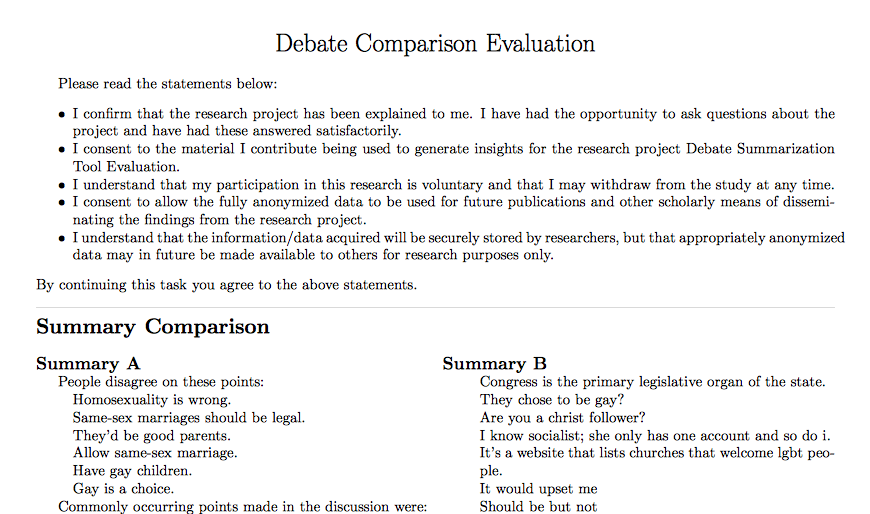
\includegraphics[width=\textwidth]{form}
  \end{frame}

  \begin{frame}{Motivations}
	\begin{center}
	  \fbox{
\includegraphics[width=\textwidth]{reddit}}

	  \fbox{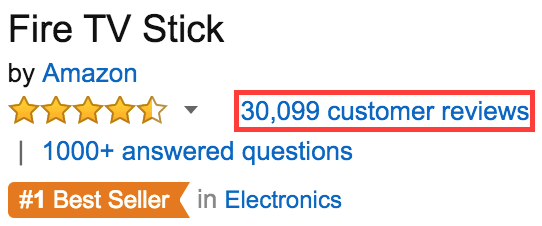
\includegraphics[width=0.5\textwidth]{fire}}

	  \fbox{
\includegraphics[width=0.6\textwidth]{indyref}}
	\end{center}
  \end{frame}

  \begin{frame}{Overview of the approach (1/2)}
	\TBox[fill=black!5]{10cm}{
	  Discussion \\[1ex]
	  \TBox[fill=black!10]{9.7cm}{
	  	Post \\[1ex]
		\TBox[fill=black!15]{9.4cm}{
		  Sentence \\[1ex]
		  \TBox[fill=green!5]{9.1cm}{
			Point \\[1ex]
			\TBox[fill=green!15]{2cm}{Extract}
			\TBox[fill=green!15]{2cm}{Verb}
			\TBox[fill=green!15]{3.95cm}{
			  Pattern \\[1ex]
			  \TBox[fill=green!25]{3.65cm}{Component}
			}
		  }
		}
	  }
	}
	\begin{itemize}
	  \item[]{\textbf{Extract:} ``\textit{A woman has rights.}''}
	  \item[]{\textbf{Verb:} have}
	  \item[]{\textbf{Pattern:} \texttt{woman.nsubj have.verb rights.dobj}}
	  \item[]{\textbf{Component:} \texttt{woman.nsubj}}
	\end{itemize}
  \end{frame}

  \begin{frame}{Overview of the approach (2/2)}
	\resizebox{\textwidth}{!}{
	  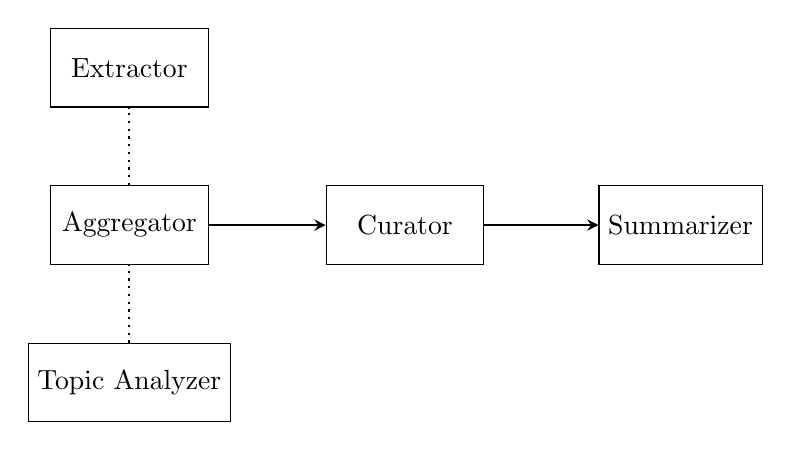
\begin{tikzpicture}[node distance=3.5cm]
		\node (agg) [service] {Aggregator};
		\node (top) [service, below of=agg, yshift=1.5cm] {Topic Analyzer};
		\node (ext) [service, above of=agg, yshift=-1.5cm] {Extractor};
		\node (cur) [service, right of=agg] {Curator};
		\node (sum) [service, right of=cur] {Summarizer};

		\draw [flow] (agg) -- (cur);
		\draw [flow] (cur) -- (sum);
		\draw[dotted] [depends] (agg) -- (ext);
		\draw[dotted] [depends] (top) -- (agg);
	  \end{tikzpicture}
	}
  \end{frame}

  \begin{frame}{Results}
    This is some content
  \end{frame}

  \begin{frame}{Further Work}
    This is some content
  \end{frame}

  \begin{frame}{Questions \& Discussion}
    This is some content
  \end{frame}
\end{document}
